\documentclass[10pt, a4paper]{report}
\usepackage[utf8]{inputenc}
\usepackage[T1]{fontenc}
\usepackage{amsmath}
\usepackage{amsfonts}
\usepackage{amssymb}
\usepackage{graphicx}
\usepackage{siunitx} % Provides the \SI{}{} and \si{} command for typesetting SI units
\usepackage{gensymb} % Degree symbol

\usepackage{hyperref}
\hypersetup{
	colorlinks=true,
	linkcolor=blue,
	filecolor=magenta,      
	urlcolor=cyan,
}

\author{Pranav Gade\thanks{notes from lectures by Dr. Somesh Kumar}}
\date{Dec. 2020 - Mar. 2020}
\title{Fundamentals of Electronic Engineering}


\begin{document}
	\maketitle
	\section*{Links}
	\begin{itemize}
		\item Email: \href{somesh@iiitl.ac.in}{somesh@iiitl.ac.in}
		\item Google Classroom: \href{https://classroom.google.com/u/3/c/MjQxNjk2NDYzMjc3}{https://classroom.google.com/u/3/c/MjQxNjk2NDYzMjc3}
	\end{itemize}
	\section*{Marking Scheme}
	\begin{itemize}
		\item Mid Sem: 30m
		\item End Sem: 70m
		\item Assignments: 30m
		\item Attendance: 10m
		\item Class performance: 10m
		\item Labs: 100m
		\item Total: 250m
	\end{itemize}
	\section*{Assignment 1}
	\begin{enumerate}
		\item how zener diode can be used as voltage regulator
	\end{enumerate}
	\newpage
	
	\chapter{Introduction}	
	\section{Basic Terms}
	\begin{itemize}
		\item \textbf{Thermal Voltage($V_t$)}: Volt equivalent of temperature $ V_t = \frac{\overline{k}T}{q} $ \\
		where\\ $\overline{k} =$  Boltzman's Constant$ = 1.381\times 10^{-23}J/\degree K  = q \times K$; \\
		$ k = 8.65 \times 10^{-5} eV/ \degree K $\\
		$ V_T = \frac{T}{11600} V$ \\
		Suppose $ T=300 \degree K $(room temp.):\\So, $ V_T = \frac{300}{11600} = 0.0258V = 26mV$
		\textbf{\item Electron Volt(eV)}: Energy gained by an electron while moving through a potential difference of 1 volt. \\
		$ 1 eV = q \times P.D. = 1.69 \times 10^{-19}C \times  1V = 1.69 \times 10^{-19}CV= 1.69 \times 10^{-19}J  $(this is K.E.)
		\item \textbf{Leakage Current($ I_0 $)}: \begin{itemize}
			\item (aka Thermally generated current) 
			\item This depends on minority Charge carrier.
			\item Never depends on applied voltage. Depends on temperature.
			\item Should be as small as possible for efficiency.
		\item\begin{tabular}{|c|c|c|}
			\hline
			& Ge & Si \\
			\hline
			$I_0$ & $\mu$A & $\eta$A \\
			\hline
		\end{tabular}
			\item Small leakage current -> no false triggering(randomly turning on)
			\item Therefore, Si is better because no false triggering.
			\item $ I_{0(T_2)}  = I_{0(T_1)}  \times  2^{\frac{T_2 - T_1}{10}}$
			\item $ I_0 $ will double every 10\degree C rise in temp(for Si, Ge)
			\item $ I_0 $ is 7\% higher for 1\degree C rise in temp.
			\item Si is better for high temp because smaller $ I_0 $, which can eliminate false triggering.
		\end{itemize}
		\item \textbf{Energy Gap($ E_g $)}:\begin{itemize}
			\item aka Band Gap, see fig. \ref{fig:energy-band-diagram}
			\begin{figure}
				\centering
				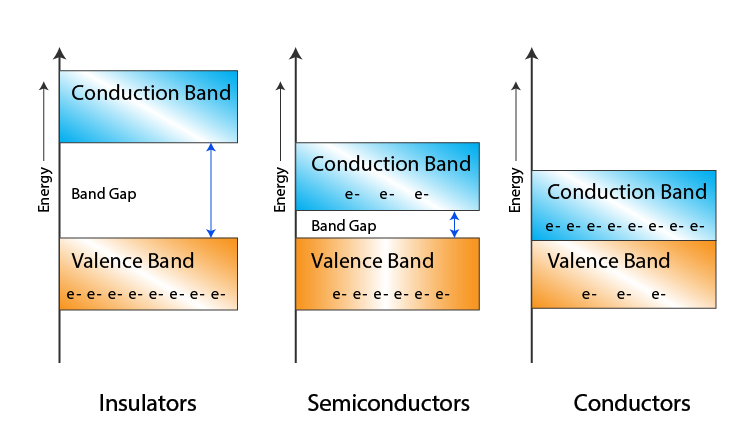
\includegraphics[width=0.7\linewidth]{img/Energy-band-diagram}
				\caption[Energy Bands]{Energy Bands}
				\label{fig:energy-band-diagram}
			\end{figure}
			
			\item Metals: $ E_G = 0 $ even at 0K. So, $ e^- $ are available even at 0K.
			\item Semiconductor: At 0K, behaves like insulator($ E_G = 1eV $). At 300K, band gap starts decreasing so conductivity increases(however, not as conductive as metals).
			\item Insulator: $ E_G = 5eV \;to\; 15 eV $ so $ e^- $ will not jump at any temp. Conductivity $\sigma = 0$ for ideal insulator; negligible practically.
			\item $ E_G \propto \dfrac{1}{temp} $
			\item $ E_{G(T)} = E_{G0} - \beta T $; ($\beta$ is $ 2.2  \times  10^{-4} $ for Ge; $ 3.6 \times  10^{-4} $ for Si)
			\item \begin{tabular}{|c|c|c|c|}
				\hline
				& Ge & Si & GaAs \\
				\hline
				$ E_{G0} $ & 0.75eV & 1.21eV & - \\
				\hline
				$ E_{G300} $ & 0.72eV & 1.1eV & 1.47eV \\
				\hline
			\end{tabular}
		\end{itemize}
		\item \textbf{Operating Temperature}: Maximum range in which the device operates. After this, melting pt. is reached and properties change. Below operating temp., band gap increases and secondary properties are seen.
			\begin{tabular}{|c|c|c|}
				\hline
				Ge & Si & GaAs \\
				\hline
				-60C to 75C & -60 to 175C & -60C to 275C \\
				\hline
			\end{tabular}
		\item \textbf{Electric Field Intensity($\epsilon$ or E)}: 
			\begin{itemize}
				\item aka field gradient
				\item $ \epsilon= \frac{dv}{dx} = $voltage/length or width
			\end{itemize}
		\item \textbf{Mobility($\mu$)}: How freely charge carriers drift(Drift $\to$ by force) in semiconductor.\\
			$\mu = \frac{Drift\; velocity(V)}{Electric\;Field\;Intensity(\epsilon)} = \frac{m^2}{V\;sec}$\\
			$\mu \propto T^{-m}$\\
			Ge: $\frac{\mu_n}{\mu_p} ~ 2.1$\\Si: $\frac{\mu_n}{\mu_p} ~ 2.6$\\
			As field intensity increases, the number of collisions increase, therefore decreasing the mobility(fig. \ref{fig:mobility-applied-electric-field-graph}) \\
			\begin{figure}
				\centering
				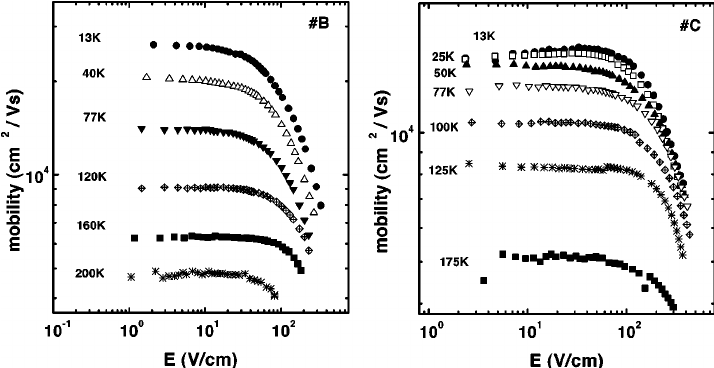
\includegraphics[width=0.7\linewidth]{img/Mobility-applied-electric-field-graph}
				\caption{graph}
				\label{fig:mobility-applied-electric-field-graph}
			\end{figure}
			\begin{tabular}{|c|c|c|c|}
				\hline
				& Ge & Si & GaAs \\
				\hline
				$\mu_n$ & $ 3800\; cm^2/V\:sec$ &  $ 1300\; cm^2/V\:sec$ &  $ 5800\; cm^2/V\:sec$ \\
				\hline
				$\mu_p$ &  $ 1800\; cm^2/V\:sec$ &  $ 500\; cm^2/V\:sec$ &  $ 400\; cm^2/V\:sec$ \\
				\hline
			\end{tabular}
			Ge is better for high freq. applications due to high Gain Bandwidth Product\\
			GaAs is best for microwave applications\\
			Si is best for switching applications.
		\item \textbf{Mass Action Law}: 
		\begin{itemize}
			\item In an extrinsic semiconductor under thermal equilibrium, the product of electrons and holes is always a constant, and is equal to the square of intrinsic concentration.
			\item $ n \times p = n_i^2 $
			\item This can be used to calculate the concentration of minority charge carriers.
			\item Therefore, $ n_p = \frac{n_i^2}{p_p} $
			\item $ majority\: carrier \propto Doping\: concentration $
		\end{itemize}
		 \item $ n_i $(Intrinsic Semiconductor Concentration):\\
		 $ n_i^2 = A_0 T^3 e^{- \frac{E_{G0}}{KT}} $, where:\\
		 $ A_0 $ is the material constant\\
		 $ T $ is the temperature\\
		 $ E_{G0} $ is the band gap
		 \item \begin{tabular}{|c|c|}
		 	\hline
		 	NTC(Negative Temp. Coeff) & PTC(Positive Temp. Coeff) \\
		 	\hline
		 	$ E_G,\ mu $ & $ n_i, v_t $ \\
		 	\hline
		 \end{tabular}
	  	 \item \textbf{Resistivity}: Specific resistance of any material($ \ohm \: m, \ohm \: cm $)\\
	  	 \begin{tabular}{|c|c|}
	  	 	\hline
	  	 	Metals & Semiconductor \\
	  	 	\hline
	  	 	Incr. with Temp. & Decr. with Temp. \\
	  	 	\hline
	  	 \end{tabular}
  	 	 \item \textbf{Conductivity}: Current carrying capacity of material($ \sigma = 1/\rho $)\\
  	 	 $\sigma = carrier\: conc \times charge \times mobility$\\
  	 	 For metals: $\sigma = n \times q \times \mu$(decreases with temp.)\\
  	 	 For semiconductors: $\sigma = nq\mu_n + pq\mu+p$ (since both $ e^- $ as well as holes contribute)(overall incr. with temp.)
  	 	 \item \textbf{Current density}: $ J = I/A \: Amp/m^2 = \sigma E $\\
  	 	 See sigma formulae from above as well
  	 	 \item \textbf{Diffusion Constant}: This a property of the material. It depends on temperature.
  	 	 \item \textbf{Diffusion Length}: The average length a carrier moves between generation and recombination. \\
  	 	 $ L = \sqrt{D\tau} $, where $\tau$ is the average lifetime\\
  	 	 $ e^- $ diffusion length $ L_n = \sqrt{D_n\tau_n} $
  	 	 \item \textbf{Concentration Gradient}: $ \frac{dn}{dx} $ is the $ e^- $ concentration gradient. $ \frac{dp}{dx} $ is holes concentration gradient.
  	 	 \item $ J_n(diff) = +q\:D_n\frac{dn}{dx}  A/cm^2$\\$ J_p(diff) = -q\:D_p\frac{dp}{dx}  A/cm^2$ \\
  	 	 $ J_{(diffusion)} = J_{n(diff)} + J_{p(diff)} $ \\
  	 	 $ I_n(diff) = J_{n(diff}) \times A $, where A is the cross sect. area\\
  	 	 Total current, $ J = J(diff) + J(drift) $ \\
   	 	 $ J_n = qD_n\frac{dn}{dx} + nQ\mu_n \epsilon $ (similar for $ j_p $)
	\end{itemize}
	\section{Einstein's Equation}
	\begin{itemize}
		\item $ \frac{D_n}{\mu_n} = V_T = kT = \frac{D_p}{\mu_p} $, where $ D $ is the Diffusion constant
		\item unit of $\frac{D}{\mu}$ is Volt
	\end{itemize}
	\section{Semiconductors}
\begin{itemize}
	\item conductivity between conductor and insulator
	\item around $ 1eV-1.5eV $
	\item Bipolar
	\item NTC
\end{itemize}
	\section{Doping}
	process of adding impurities in SC. doping $\uparrow$, carrier conc.$\uparrow$, conductivity $\sigma$$\uparrow$
	\begin{enumerate}
		\item Trivalent/Acceptor impurities: B, Al, Ga, Sn
		\item Pentavalent/Donor impurities: P, As, Sb, Bi
		\item doping is based on conc. of impurities.
		\begin{enumerate}
			\item Moderate Doping: 1/[$ 10^6 \; to\; 10^8 $] $\rightarrow$ $ P\; N $
			\item Light Doping: 1/[$ 10^{11}$] $\rightarrow$ $ P^-\; N^- $
			\item High Doping: 1/[$ 10^3 $] $\rightarrow$ $ P^+\; N^+ $
		\end{enumerate}
		\item 1/$ 10^8 $ converts intrinsic to extrinsic \\
		1/$ 10^8 $ doping in Ge $\rightarrow$ $\sigma$ $\uparrow$ 12 times \\
		1/$ 10^7 $ doping in Ge $\rightarrow$ $\sigma$ $\uparrow$ 120 times
		\item Doping can be homogeneous(same throughout) or non homogeneous(different at diff. points)
		\item Ge-Si crystal: intrinsic at 300K
	\end{enumerate}
	\section{Extrinsic SC}
	aka doped SC/Impurity SC/Artificial SC/degenerate SC/Compensated SC \\
	\subsection{N type or Donor SC}
	\begin{itemize}
		\item Pentavalent
		\begin{figure}[h]
			\centering
			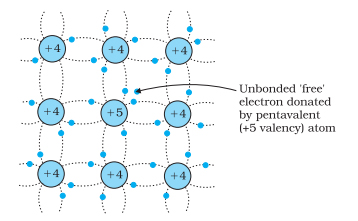
\includegraphics[width=0.7\linewidth]{img/Extrinsic-semiconductor-1}
			\caption{N-type SC}
			\label{fig:extrinsic-semiconductor}
		\end{figure}
		\begin{figure}[h]
			\centering
			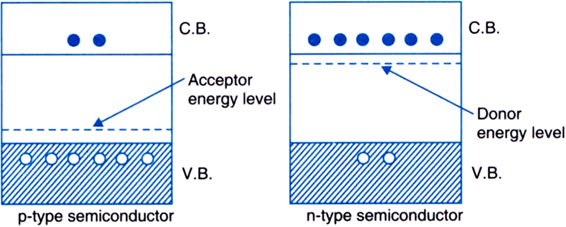
\includegraphics[width=0.7\linewidth]{img/extrinsic_band_gap}
			\caption{SC band gap at 300K \\ Donor energy lvl is 0.01 eV for Ge, 0.05 eV for Si}
			\label{fig:extrinsic-band-gap}
		\end{figure}
		\item As temp $\uparrow$ from 0K to 300K, 5th $ e^- $ move from donor lvl to conduction(fig. \ref{fig:energy-band-diagram})
		\item P type SC is represented with (+) because it has pentavalent atoms that have lost their $ e^- $
	\end{itemize}
	\subsection{P type or Acceptor SC}
	\begin{itemize}
	\item Trivalent
	\begin{figure}[h]
		\centering
		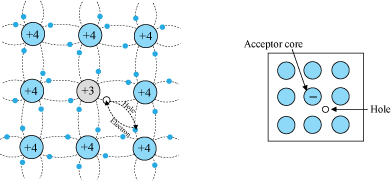
\includegraphics[width=0.7\linewidth]{img/p_type}
		\caption{P-type SC}
		\label{fig:ptype}
	\end{figure}
	
	\item See fig. \ref{fig:extrinsic-band-gap} for band gaps
	\item P type SC is represented with (+) because it has pentavalent atoms that have lost their $ e^- $
	\item Holes act as majority charge carrier. $ p>n_i $
	\item $ N_D + p = N_A + n $ \\ $ n + N_A = p $ \\ $ p \approx N_A $
	\end{itemize}
	\textbf{Q1:} Calculate the intrinsic conductivity \& intr. resistivity of Ge at 300K. $ n_i = 2.5 \times  10^{13} atoms/cm^3,\mu_n = 3800 cm^2/V\: sec, \mu_p = 1800 cm^2/V\: sec $ \\
	Ans: 
	$\sigma_i = n_i q [\mu_p + \mu_n] = 0.0222 $\\
	\textbf{Q2:} How many times $\sigma$ $\uparrow$ in the sc due to doping, IR = $ 1:10^7 $ Assume total no. of atoms = $ 4.421 \times 1-^{22} /cm^3 ; n_i = 2.5 \times 10^{13} / cm^3$\\
	Ans: 
	$ \frac{\sigma_n}{\sigma_i} = 120 times $\\
	\textbf{Q3:} A pure SC is doped with acceptor impurities to extent of 4 impurity atoms for every 1 million of atoms. calculate $\sigma$\\
	
	\subsection{Compensated SC} Acceptor as well as Donor added
	\begin{enumerate}
		\item if $ N_A = N_D \implies $ intrinsic
		\item if $ N_A > N_D \implies $ P type compensated SC
		\item if $ N_A < N_D \implies $ N type compensated SC
	\end{enumerate}
	\subsubsection{Equation for conc. of $ e^- $ in the conduction band of Intrinsic SC}
	The equation for $ e^- $ conc. in the CB of intrinsic SC is: $ n = N_C \: e^{-\frac{E_C-E_F}{kT}} $, where $ N_C $ is the material const, a fxn of temp.($ N_C \propto T^{3/2} $)\footnote{$ N_C = 2(\frac{2\pi k T M_n}{h^2})^{3/2} $; in Si, $ M_C = 1.08\times m $, where $ m $ is the rest mass of $ e^- = 9.1\times 10^{-31}kg $}

	\subsubsection{Fermi Level/Energy $ E_F $} is the max. energy posessed by $ e^- $ at 0K, see fig. \ref{fig:energy-brands-in-silicon}
	\begin{figure}[h]
		\centering
		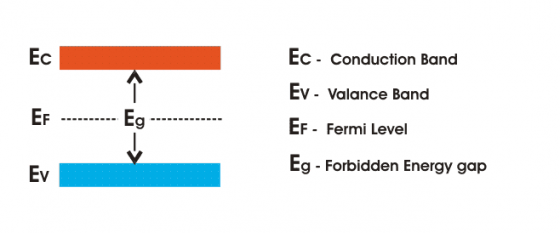
\includegraphics[width=0.7\linewidth]{img/energy-brands-in-silicon}
		\caption{Energy Bands of Silicon}
		\label{fig:energy-brands-in-silicon}
	\end{figure}
	
	\subsubsection{Equation for conc. of holes in the valence band of Intrinsic SC}
	$ p = N_V \: e^{-\frac{E_F-E_V}{kT}} $, where $ N_V $ is the material const, a fxn of temp.($ N_C \propto T^{3/2} $)\footnote{$ N_V = 2(\frac{2\pi k T M_p}{h^2})^{3/2} $; in Si, $ M_V = 0.56\times m $}
	
	\subsubsection{Eqn. of intrinsic conc. $ n_i $}
	1: $ n = N_C \: e^{-\frac{E_C-E_F}{kT}} $\\
	2: $ p = N_V \: e^{-\frac{E_F-E_V}{kT}} $\\
	Multiply 1 and 2: 
	$ np = N_C N_V \: e^{-\frac{E_C-E_V}{kT}} $\\
	$ np = N_C N_V \: e^{-\frac{E_G}{kT}} $\\
	$ A_0 = N_CN_V  = 4(\frac{2\pi k}{h^2})^3 (M_NM_P)^{3/2} T^3$\\
	mass action law: $ n_i^2 = np $\\
	$\therefore , n_i^2 = A_0 T^3e^{-\frac{E_{G0}}{kT}}$
	
	\subsubsection{Mass action law}
	under \textbf{thermal equilibrium}, $ np = N_cN_v e^{-\dfrac{E_g}{kT}} = n_i^2 $
	\subsection{Degenerate SC:} minority conc. is negligible bcoz v high majority conc\\
	
	\subsection{Effect of temp. on $ \sigma $ in extrinsic SC}
	see fig. \ref{fig:effect-of-temp}\\
	Above Curie temp $ T_C $, starts behaving like intrinsic SC.
	\begin{figure}[h]
		\centering
		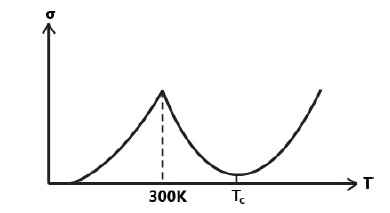
\includegraphics[width=0.7\linewidth]{img/effect-of-temp}
		\caption{Dependence of $ \sigma $ on T. $ T_C $ is the Curie temp.}
		\label{fig:effect-of-temp}
	\end{figure}
	

	\subsection{Effect of temp. on $ \sigma $ in intrinsic SC:}
	In intrinsic SC, $ n = p $ \\
	$ N_c  e^{-\frac{E_c-E_F}{kT}}  = N_v e^{-\frac{E_F-E_V}{kT}}$ \\
	$ ln \frac{N_c}{N_v}  = \frac{E_c+E_v-2E_F}{kT}$ \\
	$ E_F = \frac{E_C+E_V}{2} -\frac{kT}{2}ln\frac{N_c}{N_v}$\\
	\begin{itemize}
		\item \textbf{Case-1 } Let $ m_p = m_n $(assumption) $ N_c = N_v $\\
		$ E_F = \frac{E_c + E_v}{2} $ 
		\item At T=0K, fermi lvl lies in middle of CB\&VB. Hole conc. is 0 in VB
		\item \textbf{At T=300K} $ E_F = \frac{E_c+E_v}{2} -\frac{kT}{2} ln \frac{N_c}{N_v}$ since $ N_c > _v $ and T > 0, fermi lvl will be lower. (see fig. \ref{fig:fermilvl})
		\begin{figure}[h]
			\centering
			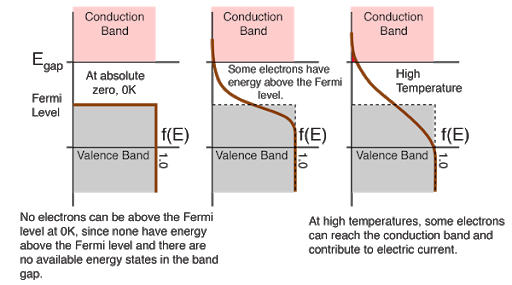
\includegraphics[width=0.7\linewidth]{img/fermi_lvl}
			\caption{}
			\label{fig:fermilvl}
		\end{figure}		
	\end{itemize}

	\subsection{Effect of temp. on $ \sigma $ in N type SC}
	$$ n \approx N_D $$
	$$ N_c  e^{-\frac{E_c-E_F}{kT}}  \approx N_D$$
	$$ ln\frac{N_C}{N_D}  = \frac{E_C - E_F}{kT}$$
	$$ E_F = E_C - kT\; ln \frac{N_C}{N_D} $$
	\begin{itemize}
		\item \textbf{Case 1} T = 0K \\
		$ E_F = E_C $ so, no holes and no $ e^- $
		\item \textbf{At 300K} $ E_F = E_C - k T\; ln \frac{N_C}{N_D} $ \\
		see fig. \ref{fig:fermilvlntype}
		\item \textbf{At more than 300K}: $ E_C > E_F $ since $\sigma$$\downarrow$ with temp \\
		so, $ E_F $ goes downward
		\begin{figure}
			\centering
			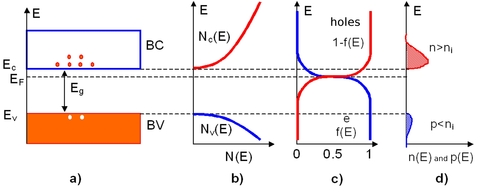
\includegraphics[width=0.7\linewidth]{img/fermi_lvl_ntype}
			\caption{}
			\label{fig:fermilvlntype}
		\end{figure}
	\end{itemize}
	\subsection{Effect of doping on $ \sigma $ in N type SC}
	$ N_D \uparrow, let \; N_D > N_C $\\
	$ E_C < E_F $
	\begin{enumerate}
		\item \textbf{if $ N_D \approx N_C $} $ E_F = E_C $
		\item \textbf{if $ N_D > N_C $} $ E_F > E_C $
		\item \textbf{if $ N_D < N_C $} $ E_F < E_C $
	\end{enumerate}
	\subsection{Effect in P type SC}
	In p type SC, $ p \approx N_A $
	$$ \therefore N_A = N_V e^{-\dfrac{E_F-E_V}{kT}} $$
	$$ \therefore ln\dfrac{N_V}{N_A}  = {\dfrac{E_F-E_V}{kT}}$$
	$$ E_F = E_V + kT \ln\dfrac{N_V}{N_A} $$
	\paragraph{Variation with temperature}
	\begin{enumerate}
		\item \textbf{T = 0K} $ \implies  E_F = E_V$
		\item \textbf{T = 300K} $ E_F = E_V + kT \ln\dfrac{N_V}{N_A} $
		\item \textbf{T > 300K} $ E_F\uparrow as \; T\uparrow $
	\end{enumerate}
	
	\paragraph{Variation with doping}
	\begin{enumerate}
		\item $ N_A \approx N_V \rightarrow E_F = E_V$
		\item $ N_A > N_V \rightarrow E_F < E_V $
		\item $ N_A < N_V \rightarrow E_F > E_V $
	\end{enumerate}
	
	\section{Hall Effect}
	Hall Effect States that If a specimen(metal/SC) carrying current $ I $ is placed in transverse magnetic field $ B $, $ E $ is induced in a direction $ \perp $ to both $ B \& I $ (fig. \ref{fig:hall-effect})
	\begin{figure}[h]
		\centering
		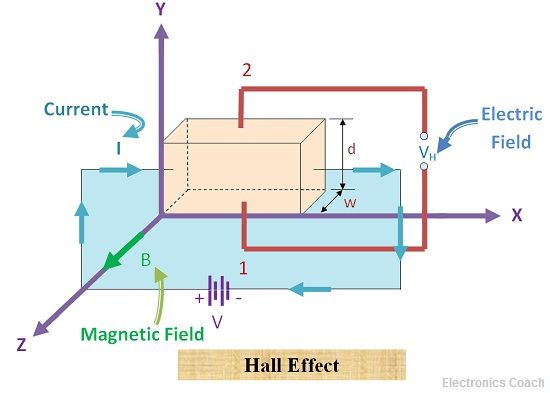
\includegraphics[width=0.7\linewidth]{img/hall-effect}
		\caption{Hall Effect}
		\label{fig:hall-effect}
	\end{figure}
	\par 
	From Hall effect, we can determine:
	\begin{enumerate}
		\item Whether the given specimen is metal/SC(intrinsic, P, N)
		\item Carrier conc.
		\item Mobility of charge carrier
		\item H, B
	\end{enumerate}
	Let $ V_H  = 2-1$ in fig. \ref{fig:hall-effect}
    \begin{itemize}
    	\item If $ V_H  <  0$ it's Metal/N-type
    	\item If $ V_H > 0$ it's P-type
    	\item If $ V_H \approx \mu V $ it's Metal
       	\item If $ V_H \approx m V $ it's SC
       	\item If $ V_H \rightarrow 0 $ it's intr. SC
    \end{itemize}
	\subsection{Field Intensity}
	Magnitude of field Intensity $ |E| = \frac{|V_H|}{d} V/m$ \\
	Hall Voltage $ V_H = Ed \; Volt $\\
	$ V_H = \dfrac{BI}{\rho w} $, where $\rho$ is the charge, $ \dfrac{1}{\rho} = R_H$ is Hall Effect const.\\
	$ V_H = \dfrac{BIR_H}{W} Volts$, or $ V_H \propto R_H $\\
	\\
	$\star$ $ \mu = \dfrac{8}{3\pi} \sigma R_H $, experimentally

	\subsection{Applications}
	\begin{itemize}
		\item Magnetic Field Meter $\rightarrow$ H
		\item Hall Effect multiplier: (I, B) $\rightarrow$ $ V_H $
	\end{itemize}
	$\star$ $ \rho $ = charge $\times$ carrier conc. ($ C/m^3 $)
	We know, $ R_H = \dfrac{1}{charge \times c.c.} $
	Therefore,
	\begin{itemize}
		\item \textbf{$ R_H < 0 $} for metals, N type SC
		\item \textbf{$ R_H > 0 $} for P type SC
		\item \textbf{$ R_H $ very large} for intr. SC
	\end{itemize}
	\subsubsection{Alternate formulae}
	$ V_H = \dfrac{BJd}{qN_D} $\\
	$ V_H = \dfrac{BJd}{qN_A} $\\
	\textbf{Question:} In a N type Sc, a sample has donor density $ N_D = 10^{21}/m^3 $. It is arranged in Hall experiment having magnetic field $ 0.2 WB.M^2 $\& the current density $ J =  500A/m^2$. Find the V generated when $ w=d=2mm $\\
	Ans: $ -1.25mV $
	
	\section{Classification of SC}
	\begin{itemize}
		\item \textbf{Direct Band Gap SC} like GaAs, GaAsP; give out 99\% light, 1\% heat
		\item \textbf{Indirect Band Gap SC} like Ge, Si; give out 1\% light, 99\% heat
	\end{itemize}


	\chapter{SC Diode}
	\begin{itemize}
		\item P-N Junction Diode
		\item \textbf{Metal SC diode} like Schottky Diode, Point contact Diode
	\end{itemize}
	\section{P-N Junction Diode}
	Formed when a bonding force is created b/w P-type and N-type SC. \\
	Some methods of fabrication are:
	\begin{enumerate}
		\item Diffusion method
		\item Alloy Junction
		\item Grown Junction
		\item Epitaxial method (epi-upon, taxial-layer)
	\end{enumerate}
	\begin{figure}[h!]
		\centering
		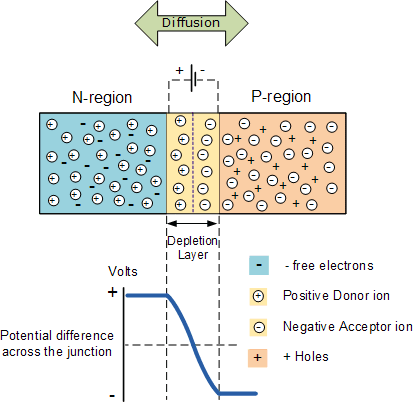
\includegraphics[width=0.7\linewidth]{img/pn-diode}
		\caption{P-N Junction Diode}
		\label{fig:pn-diode}
	\end{figure}

	\subsection{$ V_0 $} Potential hill/Barrier Potential/Barrier Voltage/Contact potential/Built-in potential/Diffusion potential\\
	$ V_0 = V_T \; ln \dfrac{N_A N_D}{N_i^2} $ \\
	therefore, $ V_0 \downarrow with\;  T \uparrow $, because $ n_i^2 \propto T^3 $ ($ V_0 \downarrow by \; 2.5mV \; for t \uparrow by \; 1K $)
	\begin{itemize}
		\item Si: 0.6 to 0.9 V (0.7V avg.)
		\item Ge: 0.1V to 0.5 V (0.2V avg.)
	\end{itemize}
	\begin{figure}
		\centering
		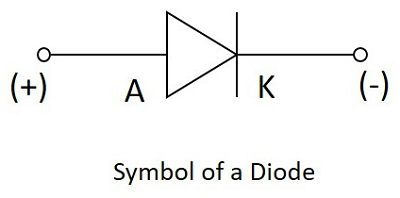
\includegraphics[width=0.2\linewidth]{img/diode_symbol}
		\caption{}
		\label{fig:diodesymbol}
	\end{figure}
	
	\subsection{Depletion Layer}
	aka Space Charge region/Transition region. Any layer in which charge carriers are absent. This contains immobile ions. \\
	Formed due to diffusion of majority charge carriers.\\
	Depletion width $ w = \sqrt{\frac{2\epsilon}{q}(\frac{1}{N_A} + \frac{1}{N_D})} $ \\
	$ \epsilon = permittivity\; in \; I/m  = \epsilon_0 \epsilon_r$\\
	$\epsilon_r(Si) = 11.7;\; \epsilon_r(Ge) =16$\\
	If $ N_A = N_D  \implies w = \sqrt{\dfrac{4\epsilon V_0}{qN_A}}$\\
	therefore, $ w \propto\dfrac{1}{\sqrt{Doping}} $\\
	Also, $ w \propto \dfrac{1}{\sqrt{Fwd.bias}} $
	
	\subsection{Forward Bias}
	As $\epsilon$ is applied, the depletion width narrows.
	\begin{figure}[h!]
		\centering
		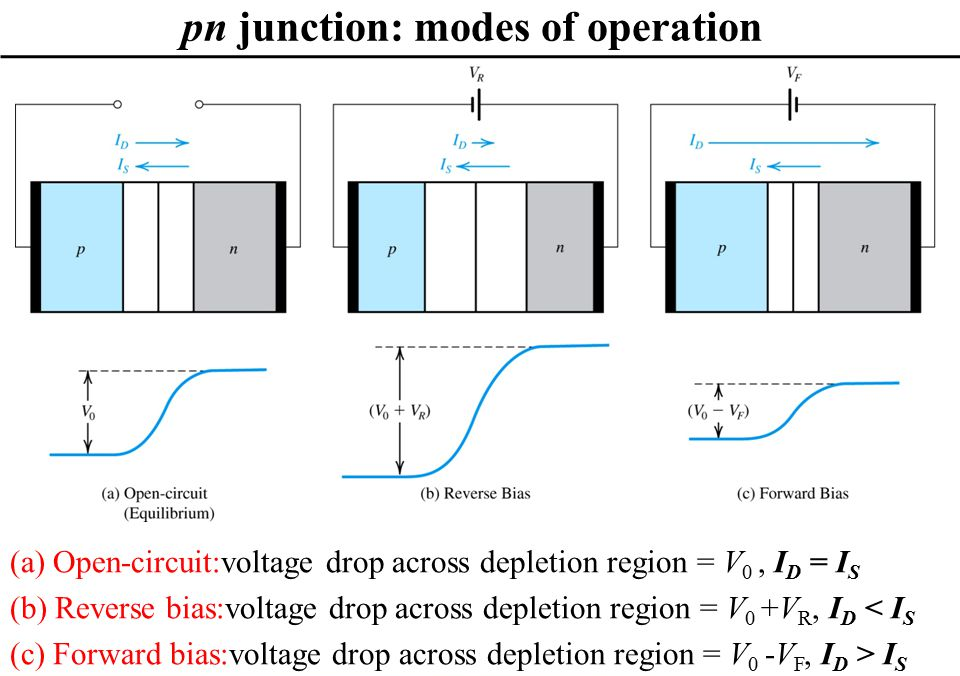
\includegraphics[width=0.7\linewidth]{img/potential-across-diode}
		\caption{}
		\label{fig:potential-across-diode}
	\end{figure}
	When $ V_D $ is the Depletion potential, $ V = V_R + V_D $\\Barrier Voltage at junction = $ V_0 - |V_D| $
	\begin{itemize}
		\item If $ V_D < V_0 $ no majority carriers cross
		\item If $ V_D \approx V_0 $, then  $ I_F \approx 0 $
		\item If $ V_D > V_0 \implies I_F  \uparrow$ 
	\end{itemize}
	$\star$ \textbf{Cut-in Voltage, or knee voltage $ V_Y $} is the min. of $ V_D $ ($ V_Y = 0.3V(for \; Ge) =0.7V(for \; Si) $) \\
	forward current\footnote{forward current is independent of T} $ I_f = I_0[ e^{V_d/\eta V_T}] $ (where $ I_0 $ is the reverse saturation current; $ V_d $ is the voltage across the diode, $\eta$ is the recombination factor or utility factor (1 for Ge, 2 for Si)) \\
	$ V_D = \eta V_T log(\dfrac{I_f+I_0}{I_0}) \approx \eta V_T log(\dfrac{I_f}{I_0}) $ \\
	$ V_D \downarrow $ by $ 2 mV $ per 1C
	
	\subsection{Reverse Bias}
	Some reverse saturation current does flow($ I_r = I_0 $). It does not matter on $ V_R $ because the concentration of minority charge carriers is very low. \\
	$ w \propto \sqrt{Reverse \; Bias} $ \\
	$ V_J = |V_{R}| +| V_0 |$ \\
	$ w = \sqrt{\dfrac{2\epsilon}{q}(\frac{1}{N_A} + \frac{1}{N_D}) V_J} $
	\begin{figure}[h!]
		\centering
		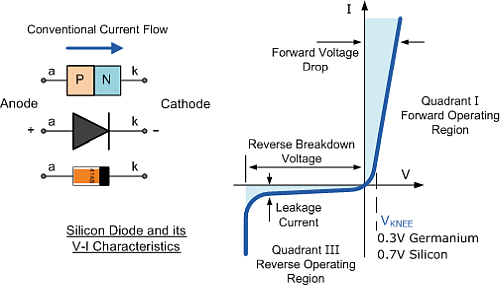
\includegraphics[width=0.7\linewidth]{img/vi-characteristics}
		\caption{V-I characteristics of diode}
		\label{fig:vi-characteristics}
	\end{figure}

	\subsection{Diode Resistance}
	\begin{itemize}
		\item forward resistance ($ R_f $): 10 $\Omega$ to 100 $\Omega$
		\begin{itemize}
			\item \textbf{DC or Static resistance}: $ R_F = \dfrac{V'}{I'} \Omega $
			\item \textbf{AC or Dynamic Resistance}: $ r = \dfrac{\Delta V_0}{\Delta I_f} = \dfrac{\eta V_T}{I_f}$\\
			Dynamic conductance(g) = $ \dfrac{1}{r}  = \dfrac{I_f}{\eta V_T} \implies g \propto I_f $
		\end{itemize}
		\item reverse resistance ($ R_r $): $ R_r > 1M\Omega $ \\
		$ I_0 \uparrow with \; T $ \\
		$ R_r \downarrow with \; T $
	\end{itemize}
	\subsection{Equivalent circuit of the diode}
		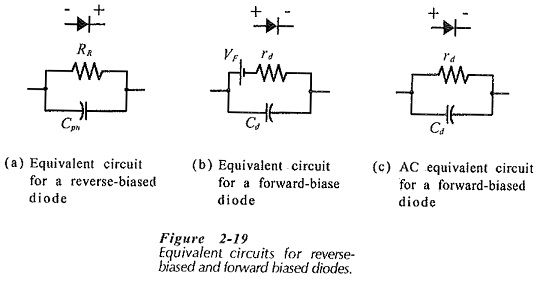
\includegraphics[width=\linewidth]{img/Equivalent-Circuit-of-Diode}
		$\star$ A fwd. bias diode can be replaced by its cut-in voltage.
	\section{Ideal/Perfect/Imaginary diode} 
	$ R_f = 0 $; $ R_r = \infty $
		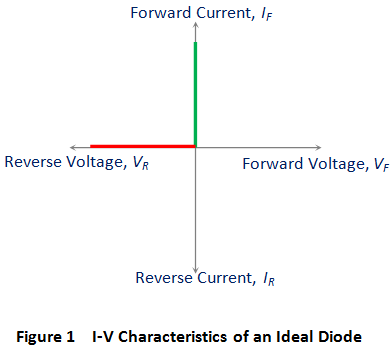
\includegraphics[width=0.7\linewidth]{img/ideal-diode-vi}
	\section{Junction Capacitance ($ C_J $)}
	in the range of pF($ 10^{-12} F $) \\
	$ C_J = C = \dfrac{A \epsilon}{w} $
	
	\subsection{Transition Capacitance($ C_T $)}
	\begin{itemize}
		\item 	aka Depletion layer capacitance aka Space Charge Capacitance
		\item $ C_T $ is the junction capacitance in R.B.
		\item $ C = \dfrac{Q}{V} = \dfrac{dQ}{dV} $
		 \item when PN jun. is RB, with a change in RB voltage w ans immobile charge carrier change, this role of change of immobile charges wet a change in RB is called $ C_T $ 
		\item Generally, $ C_T \propto V^{-n} $ where n is graded coeff., V is applied RB voltage.
	\item n = 1/2 : step graded/abrupt pn diode \\
		n = 1/3 : linear graded \\
		n = 1/2.5 : diffused PN Junction (pls confirm is it 1/3.5)
	\end{itemize}	
	\subsection{Diffusion capacitance $ C_d $}
	\begin{itemize}
		\item $ C_d \propto\sqrt{Dopin}g \propto \sqrt{F.bias}$
		\item $ C_d = \tau h $
		\item $ C_d $ will appear only at high freq. applications.
		\item $ C_d > C_T$ always 
	\end{itemize}
	
	\section{Step graded diode or Abrupt PN Junction Diode}
		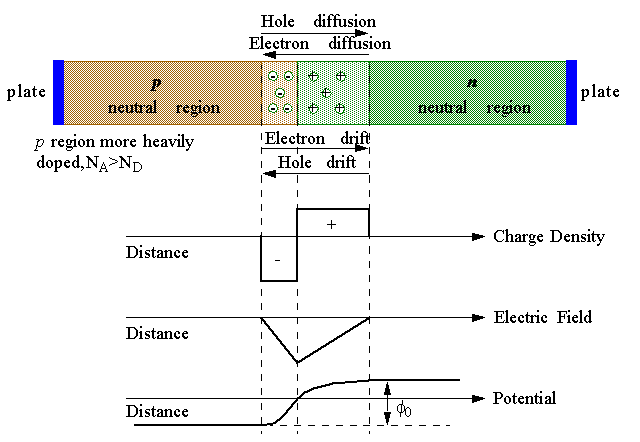
\includegraphics[width=0.7\linewidth]{img/step-graded-diode}
	\begin{itemize}
		\item $ \dfrac{W_N}{W_P}  =  \dfrac{N_A}{N_D} $
		\item less common formula: $ \dfrac{W_N}{W_P}  =  \dfrac{N_A^{1/2}}{N_D^{1/2}} $
	\end{itemize}

	\subsection{Numericals}
	\begin{enumerate}
		\item \textbf{Find the forward current of GE diode operating at room temp when fwd. voltage is 100mV; $ I_0 = 20\mu A $ }\\
		$ I_f = I_0[ e^{V_d/\eta V_T}]  = 0.936mA$
		\item \textbf{A Si diode has time const 25 ns at room temp; $ I_F = 5mS $ Find $ C_d $} \\
		$\rightarrow$ $ C_d = \tau g; g = \dfrac{I_f}{\eta V_T} $ \\
		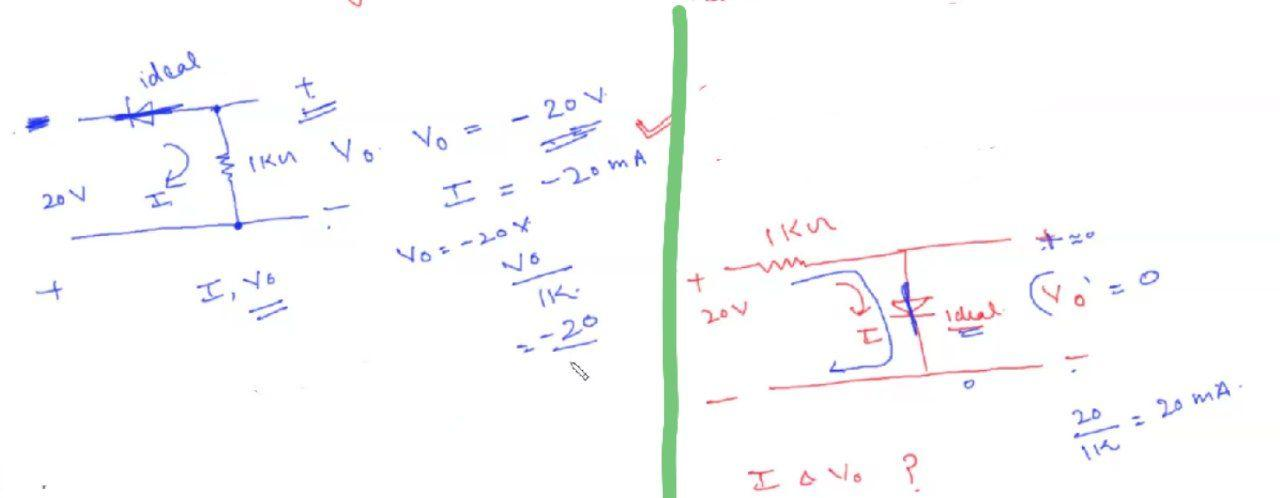
\includegraphics[width=\linewidth]{img/numericals 2nd jan}
	\end{enumerate}

	\section{Zener Diode}
	\begin{itemize}
		\item 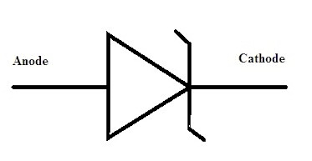
\includegraphics[width=0.5\linewidth]{img/zd symbol}
		\item 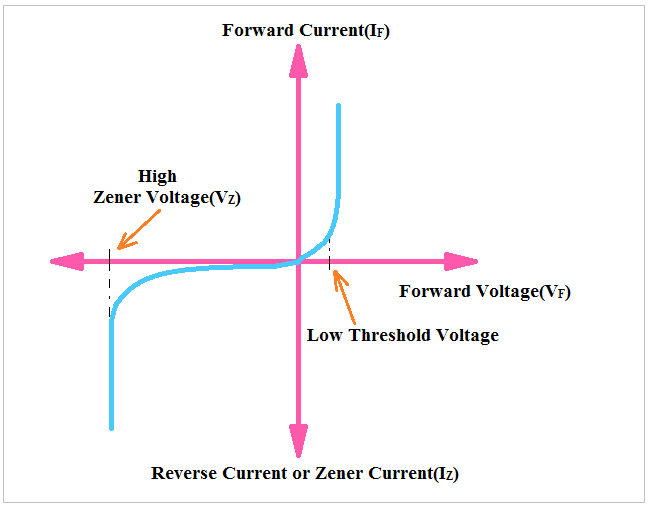
\includegraphics[width=\linewidth]{img/Zener diode characteristics}
		\item Normal diode doping $\rightarrow 1: (10^6 - 10^8)$ \\ Zener diode doping $\rightarrow 1: 10^5$
		\item By $\uparrow$ or $\downarrow$ the doping lvl. we can change the sc properties
		\item operated in rb
		\item ZD is breakdown diode because operated beyond $ V_{br} $
		\item Si is used
		\item In F.B. ZD acts like a normal diode
		\item used in constant voltage device and voltage regulators.
		\item $ R_z = \dfrac{\Delta V_z}{\Delta I_z} $ \\ in ideal case, $ R_z = 0 $ and $ V_z = V_{br} $
	\end{itemize}
	\subsection{Equivalent ckt}
	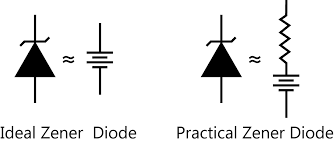
\includegraphics{img/zd equivalent}
	\subsection{Zener breakdown phenomenon}
	\begin{itemize}
		\item $ w \propto \dfrac{1}{\sqrt{Doping}} $ and $ E \propto\dfrac{1}{w} $
		\item Zener breakdown occurs due to large electric field intensity
		\item $ V_{br} < 6V \implies  $ for Zener breakdown
		\item ZB occurs due to tearing off / rupturing of covalent bond in depletion region
	\end{itemize}
	\subsection{Avalanche breakdown}
	\begin{itemize}
		\item Chain rxn, due to $ e^- $ multiplication
		\item $ V_{br} > 6V \implies  $ Avalanche breakdown
		\item Multiple collisions b/w electron and ions in the depletion region
		\item due to impact ionization
		\item In a lightly doped diode breakdown is due to avalanche effect
		\item PTC : T $\uparrow$ $ \implies $ V $\uparrow$(as mean free path decr. due to incr. collisions)
	\end{itemize}
	
	\section{LED}
	\begin{itemize}
		\item Light emitting diode
		\item 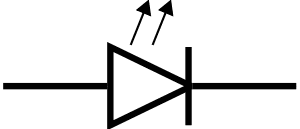
\includegraphics[width=0.2\linewidth]{img/led symbol}
		\item made frm GaAs
		\item electro-luminescence: e-h pair combine, energy is released
		\item colors depend on the wavelength and on dopant: $ \lambda = \dfrac{1.24}{E_g} $
		\item below (say, for GaAs) 1.3V, led will not glow\\ above 3.3V, it will burn out after a few seconds.
		\item $ I_f $ is 10mV (implied)
		\item response time: how long it takes to turn on and off after having the signal applied, in order of $ \mu s $
		
	\end{itemize}
	\section{Photodiode}
	\begin{itemize}
		\item photosensitive device
		\item 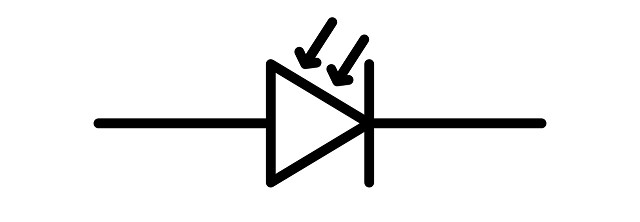
\includegraphics[width=0.2\linewidth]{img/photodiode symbol}
		\item is normal diode plus photosensitive coating like CdS, Se, ZnS
		\item always in reverse bias
		\item doping is less so depletion layer width is more
		\item works on photoconductive effect.
		\item dark current $ I_D $ is the relatively small electric current that flows even when no photons are entering the device
		\item $ I_{photon} > I_D $
		\item $ I_{total} =  I_{photon} + I_D $
		\item 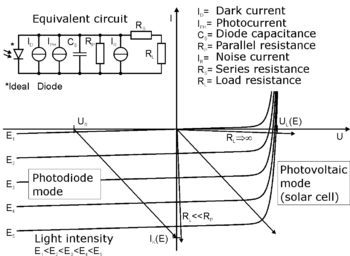
\includegraphics[width=\linewidth]{img/photodiode graph}
	\end{itemize}
	\subsection{Avalanche PD}
	Used for high current capacity
	\subsection{Tunnel Diode}
	\begin{itemize}
		\item by Japanese Esaki in 1948
		\item 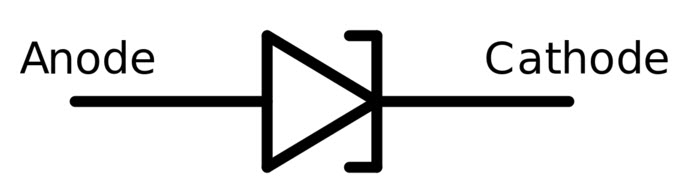
\includegraphics[width=0.2\linewidth]{img/Tunnel-Diode}
		\item made from GaAs
		\item exhibits tunneling effect hence called tunnel diode
		\item fastest diode
		\item $ w \propto \dfrac{1}{\sqrt{Doping}} $
		\item doping is highest at 1/10$ ^3 $ ratio. Hence, w is less
		\item switching time is pico seconds
		\item smaller in size, easy to fabricate, negligible internal power consumption, low noise
		\item 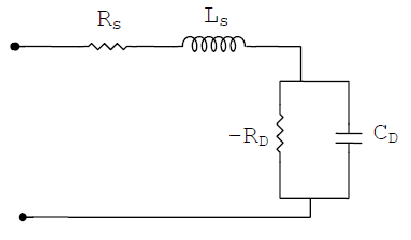
\includegraphics{img/Equivalent-circuit-of-Tunnel-diode}
		\item negative resistance: due to tunneling
		\item 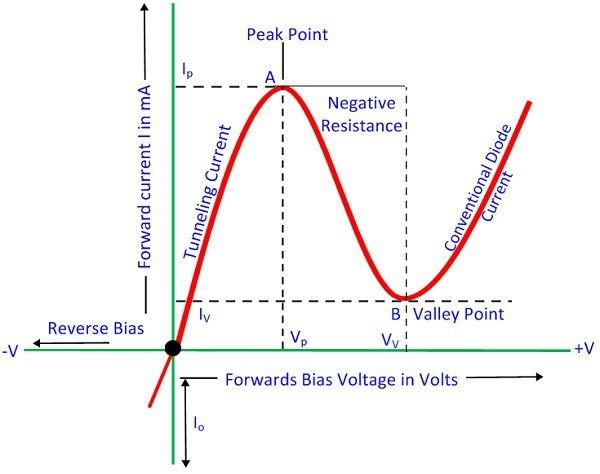
\includegraphics[width=\linewidth]{img/Tunnel-Diode-I-V-Characteristics} \\
		$ I_P $ = Peak current \\ $ I_V $ = Valley current
		\item GaAs is used because $ \dfrac{I_P}{I_V}  = 50$ (7.5 in Ge, 2.5 in Si)
		\item exhibits triple valued property: some $ I+x $ can be obtained thrice as long as $ I_V < I_x < I_P $
		\item used in relaxation oscillators, sawtooth voltage generator, Cathode Ray Oscillator
	\end{itemize}

	\section{Clipper and Clamper circuit}
	Clippers are networks that employ diodes to 'clip' away a portion of an input signal without distorting the remaining portion of the waveform. For example, in single diode rectifiers.
	\subsection{Series clipper circuit}
	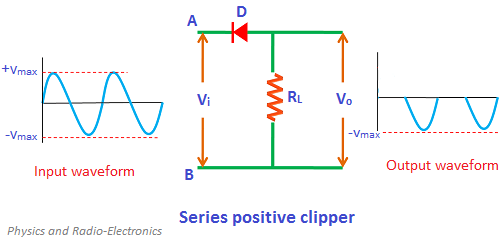
\includegraphics[width=\linewidth]{img/positiveseriesclipper}	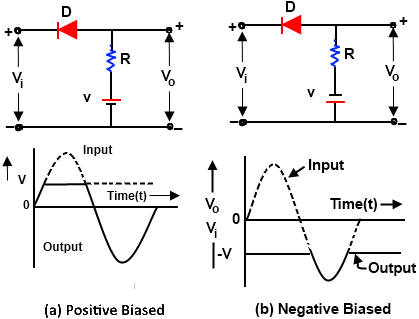
\includegraphics[width=\linewidth]{img/series-positive-clipper-with-bias}
	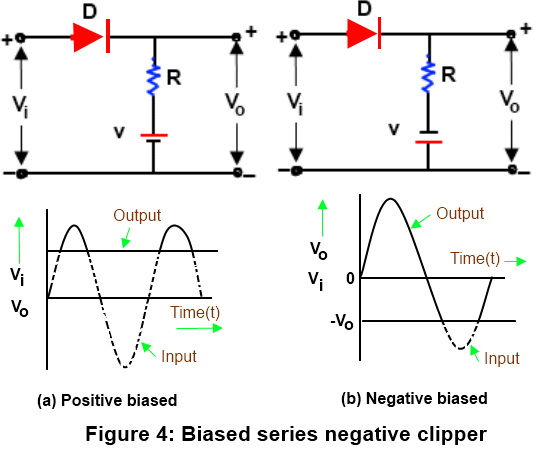
\includegraphics[width=\linewidth]{img/series-negative-clipper-with-bias}
	\subsection{Parallel clipper circuit}		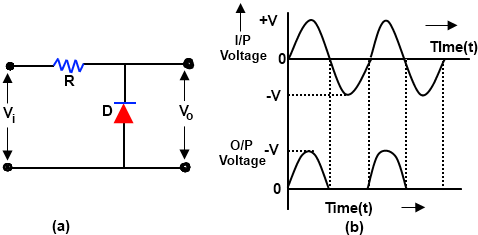
\includegraphics[width=\linewidth]{img/shunt-parallel-nagative-clipper}
	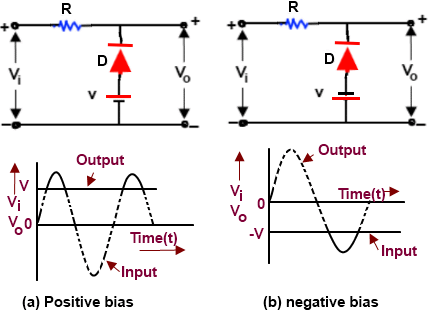
\includegraphics[width=\linewidth]{img/bias-shunt-parallel-nagative-clipper}
	
	\subsection{Clamper circuit}
	A clamper is a network constructed of a diode, a resistor, and a capacitor that shifts a waveform to a different DC level without changing the appearance of the applied signal.
	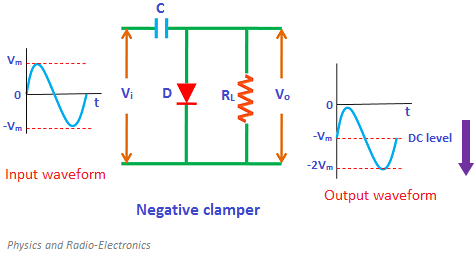
\includegraphics[width=\linewidth]{img/negativeclamper}
	\begin{enumerate}
		\item in fwd bias, capacitor will charge instantaneously
		\item Assume that the period when diode is off the capacitor held on its established lvl.
	\end{enumerate}
	A good resource: \href{http://www.physics-and-radio-electronics.com/electronic-devices-and-circuits/rectifier/clampercircuits.html}{http://www.physics-and-radio-electronics.com/electronic-devices-and-circuits/rectifier/clampercircuits.html}
	
	\subsection{Rectifier}
	AC signal to DC signal.\\
	$\star$\textbf{Peak Inverse voltage/Peak Reverse Voltage}: The voltage that must not be exceeded in reverse bias region(a property of the specific diode)
		\subsubsection{Half wave rectifier}
		$ V_{DC} =  \dfrac{V_{max}}{\pi}  = 0.318 V_{max} $
		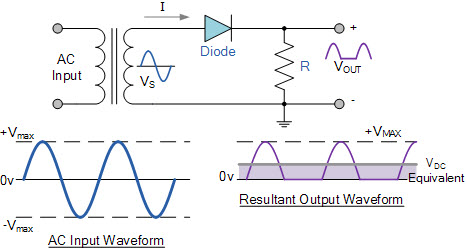
\includegraphics[width=\linewidth]{img/half rectifier}
		\\
		Because the knee voltage is non 0 in non ideal cases, the waveform looks like: \\
		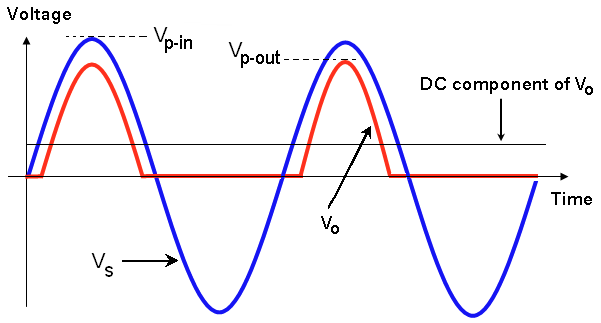
\includegraphics[width=0.5\linewidth]{img/half rectifier waveform} \\
		In this case, 		$ V_{DC} = \dfrac{V_{max} - V_K}{\pi}  = 0.318 (V_m - V_K)$\\
		$$ Efficiency\ of\ Half\ rectifier = \dfrac{DC\ power\ output}{AC\ power\ input} $$
		$$\eta = \dfrac{(\dfrac{I_m}{\pi})^2 \times R_L}{(\dfrac{I_m}{2})^2(r_f + R_L)}$$ (where $ r_f  $ is diode voltage)
		$$ \eta = \dfrac{0.406}{1+\dfrac{r_f}{R_L}} $$
		
		\subsubsection{Full wave rectifier}
		\begin{enumerate}
			\item \textbf{Bridge Network}
			\item \textbf{Center Tap Transformer}
		\end{enumerate}
		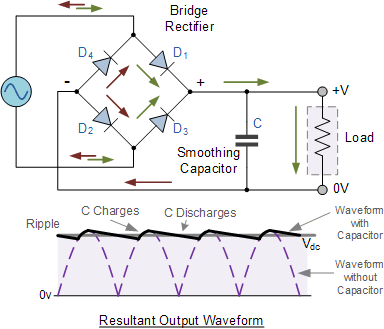
\includegraphics[width=\linewidth]{img/full rectifier}

	\chapter{Transistors}
	Transfer + Resistor
	\section{BJT(Bipolar Junction Transistor)}
		\begin{itemize}
			\item Both $ e^- $ and holes are involved in flow of electricity
			\item made in 1947 by William Schokley
			\item used as amplifiers
			\item is a CCD(Current controlled Device)
			\item 3 terminals - Emitter(emits $ e^- $), Base(in b/w E and C), Collector(collects $ e^- $)
			\item Emitter is highly doped
			\item Base is lightly doped(to reduce recombination, so that $ e^- $ can flow to collector easily) and small(to reduce transit time\footnote{time taken to move from emitter to collector})
			\item Base is the region where transistor action takes place
			\item Collector is moderately doped and large(to collect $ e^- $)
			\item Leakage current also flows(due to minority cc)
			\item therefore noisy device
			\item Thermal stability is less
			\item \textbf{Types of BJTs} \\
				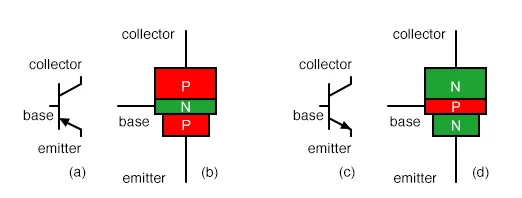
\includegraphics[width=0.9\linewidth]{img/bjt types}
			\item arrows always show direction of current flow
			\item in npn: current due to majority $ e^- $ \\in pnp: current due to majority holes
			\item Operating cases: \\
				\begin{enumerate}
					\item $ J_{EB} $ as well as $ J_{BC} $ reverse biased: negligible current flow (off switch)
					\item $ J_{EB} $ as well as $ J_{BC} $ forward biased: very large current (on switch)(coz both in fwd bias`)
					\item $ J_{EB} $ forward, $ J_{BC} $ reverse biased: Forward active region - medium current
					\item $ J_{EB} $ reverse, $ J_{BC} $ forward biased: Reverse active region - used rarely
				\end{enumerate}
		\end{itemize}
	\subsection{npn transistor}
		\begin{itemize}
			\item current due to majority $ e^- $
			\item only when $ J_E $ is FB and $ J_C $ is RB, then transistor is active
			\item 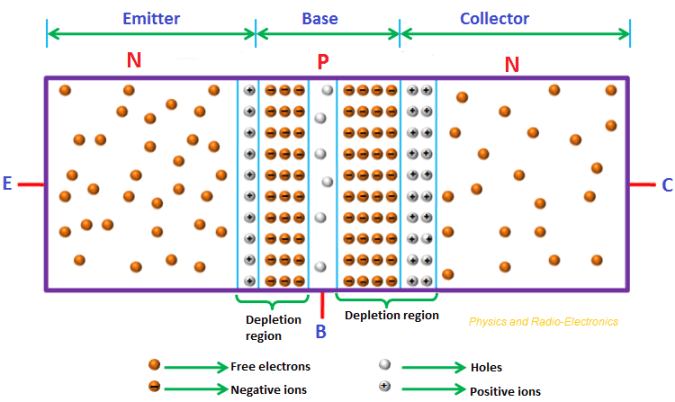
\includegraphics[width=0.8\linewidth]{img/npntransistor}
		\end{itemize}
	\subsubsection{Operation}
	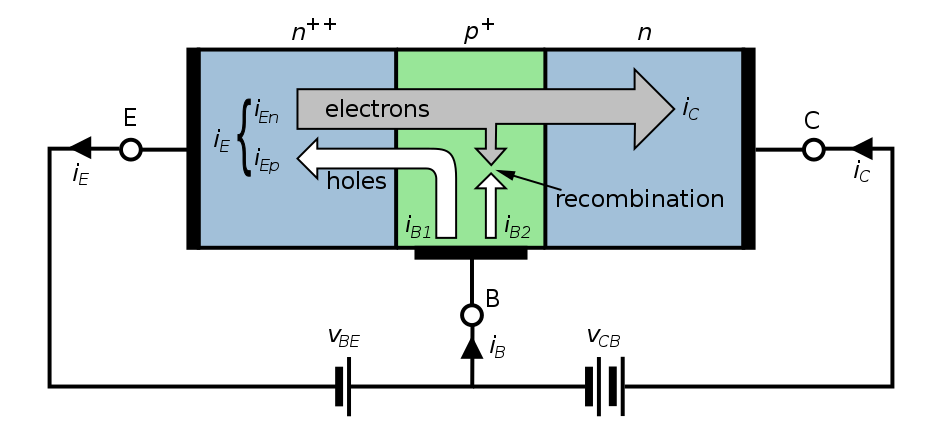
\includegraphics[width=\linewidth]{img/bjt basic op}\\\\
	when Emitter is connected to -ve, $ e^- $ move from E to B(since in forward bias). Experimentally, 5-6 $ e^- $ out of 100 recombine in base region. Now, Collector is connected to +ve. Since $ e^- $ are minority cc in Base, they will be favored to cross the base-collector reverse biased depletion region. 95-96\% $ e^- $ cross to the collector. \\
	(in the diagram) $ V_{BE} << V_{CB} $\\
	$ I_{C0} $ is the drift current due to minority cc\\
	$ I_E \ or\ I_C $ is diffusion current\\
	$ I_B $ is due to recombination
	\subsection{pnp transistor}
	\href{https://www.physics-and-radio-electronics.com/electronic-devices-and-circuits/transistors/bipolarjunctiontransistor/pnptransistor.html}{https://www.physics-and-radio-electronics.com/electronic-devices-and-circuits/transistors/bipolarjunctiontransistor/pnptransistor.html}
	
	\section{Diode equivalent circuit of Transistor}
	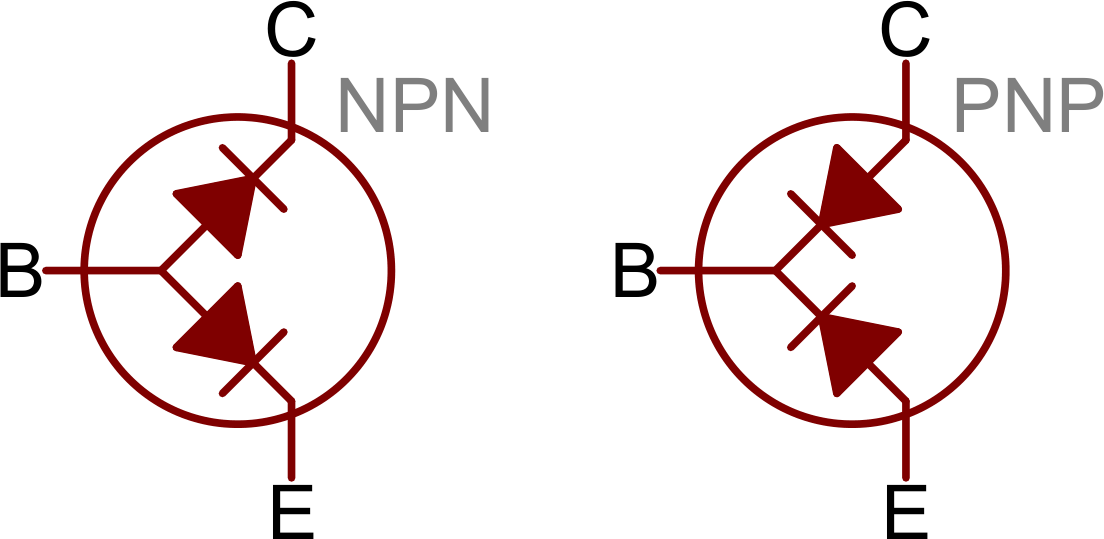
\includegraphics[width=0.6\linewidth]{img/transistors diode equivalent}
	\section{Transistor Configurations or Connections}
	\begin{tabular}{|c|c|c|c|}
		\hline
		Configuration & Input & Output & Reference \\
		\hline
		CB & E & C & Base ref \\
		\hline
		CE & B & C & Emitter \\
		\hline
		CC & B & E & Collector \\
		\hline
	\end{tabular} \\
	\textbf{Input characteristics} $ V_{o/p} $ constant\\
	\textbf{Output characteristics} $ I_{i/p} $ constant
	
	\subsection{Common Base Connection}
	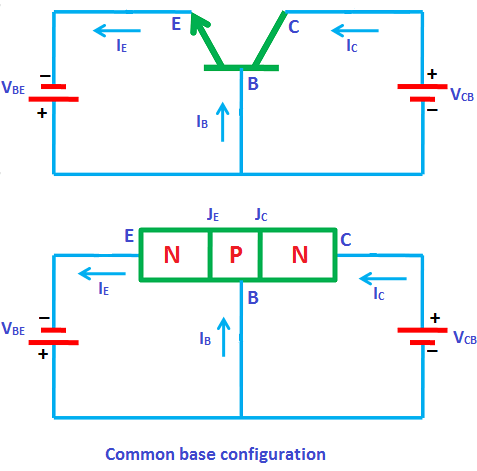
\includegraphics[width=0.8\linewidth]{img/npn cb} \\
	$\star$ current amplification factor $$ \alpha = \dfrac{\Delta I_C}{\Delta I_E} \rvert_{V_{CB = constant}}$$
	DC values considered: $ I_C = \alpha I_E $
	$$I_C = \alpha I_E + I_{CBO}$$
	$ I_{CBO} $ is the leakage current when $ I_E = 0 $
	$$I_C = \alpha (I_C + I_B)+I_{CBO}$$
	$$I_C= \dfrac{\alpha}{1-\alpha}I_B + \dfrac{I_{CBO}}{1-\alpha}$$
	
	\subsubsection{Input characteristics}
	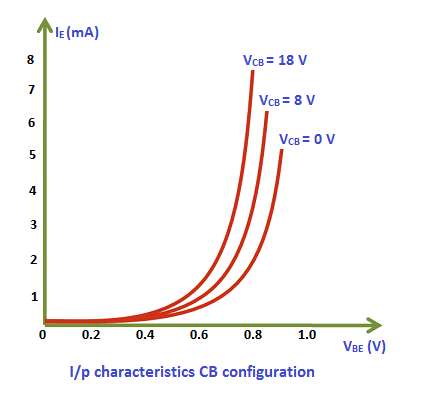
\includegraphics[width=0.6\linewidth]{img/inputcharacteristicscbconfiguration}
	\subsubsection{Input resistance}
	at const $ V_{CB} $
	$$r_i = \dfrac{\Delta V_{EB}}{\Delta I_E} $$
	lowest among all configs $\approx 100 \Omega$
	\subsubsection{Output characteristics}
	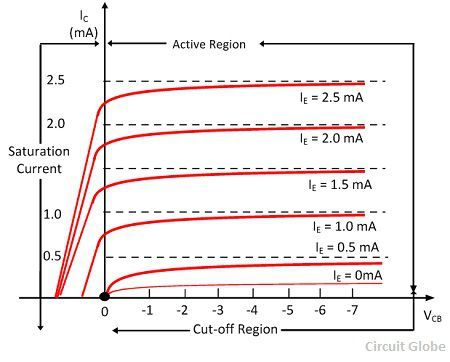
\includegraphics[width=0.6\linewidth]{img/oputputcharacteristicscbconfiguration}
	\subsubsection{Output resistance}
	at const $ I_E $
	$$r_o = \dfrac{\Delta V_{CB}}{\Delta I_C} $$
	$ r_o \approx 450 k\Omega $
	\subsection{Base width modulation/Early effect}
	As $ V_{CB} $ $\uparrow$ $ w $ in Base $\downarrow$ so recombination $\downarrow$ so base current $\downarrow$ so $ I_E \& I_C $ $\uparrow$
	\subsection{Common Emitter Configuration}
	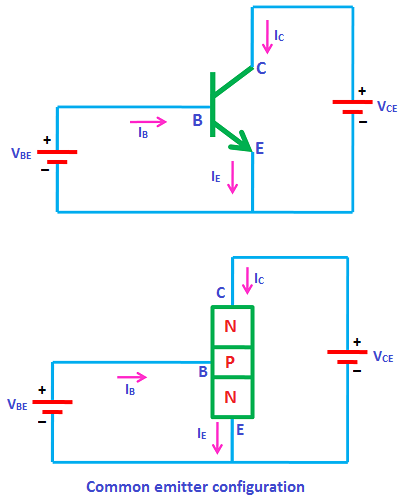
\includegraphics[width=0.8\linewidth]{img/commonemitterconfiguration}
	\begin{itemize}
		\item o/p taken from collector
		\item $\beta$ is gain
		\item Mainly used for amplification purpose
		\item $$I_E = I_B + I_C$$ 
				$$I_C = \alpha I_E + I_{CBO}$$
				$$I_C = \alpha (I_B + I_C) + I_{CBO}$$
				$$I_C(1-\alpha) = \alpha I_B +I_{CBO}$$
				$$I_C = \dfrac{\alpha}{1-\alpha}I_B + \dfrac{I_{CBO}}{1-\alpha}$$
				$$\beta = \dfrac{\Delta I_C}{\Delta I_B} = \dfrac{I_C}{I_B} $$
				$$\alpha = \dfrac{I_C}{I_E} $$
				$$I_E = I_B + I_C$$
				$$ \beta = \dfrac{\alpha}{1-\alpha} $$
				$$\alpha = \dfrac{\beta}{1+\beta}$$
				$$\therefore I_C = \beta I_B + (1+\beta) I_{CBO}$$
				$$I_{CEO} = (1+\beta) I_{CBO}$$
				$$\therefore I_C = \beta I_B + I_{CEO} $$
	\end{itemize}
	\subsubsection{Input Characteristics}
	$$r_i = \dfrac{V_{BE}}{I_B}$$\\
	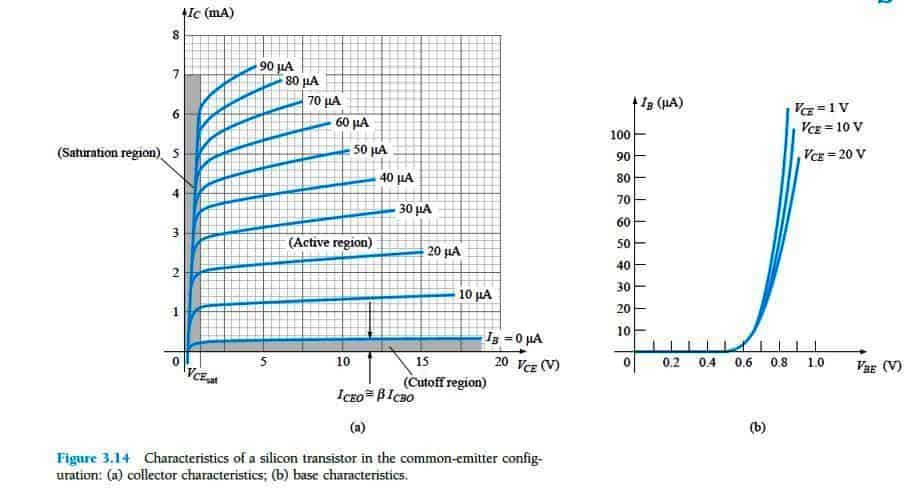
\includegraphics[width=\linewidth]{img/oputputcharacteristicsceconfiguration}\\\\
	medium/lower resistance $\approx 750 \Omega$
	\subsubsection{Output Characteristics}
	see fig. above
	$$r_o = \dfrac{\Delta V_{CE}}{\Delta I_C}$$
	$ r_o \approx 45 k\Omega $
	\subsection{Common Collector Configuration}
	$$\gamma = \dfrac{\Delta I_E}{\Delta I_B}$$
	$$\gamma = 1 + \beta = \dfrac{1}{1-\alpha}$$
	\subsubsection{Input Characteristics}
	maximum resistance $\approx 750 k\Omega$
	\subsection{}
	$$ I_f = I_0e^{\dfrac{V_d}{\eta V_T}} $$
	$$ I_e = I_{CO}e^{\dfrac{V_{BE}}{\eta V_T}} $$
	where $ V_{BE} $ is 0.7 for Si, 0.2 for Ge
	$$ P = |I_C| V_{CE} $$
	\subsubsection{Transistor as amplifier in CE}
	In positive input cycle, FB across the EB jxn or $ J_E $ $\uparrow$ \& more more $ e^- $ will flow, collector current $\uparrow$ \& potential across $ R_C $ $\uparrow$ \& opposite happens in -ve cycle.
	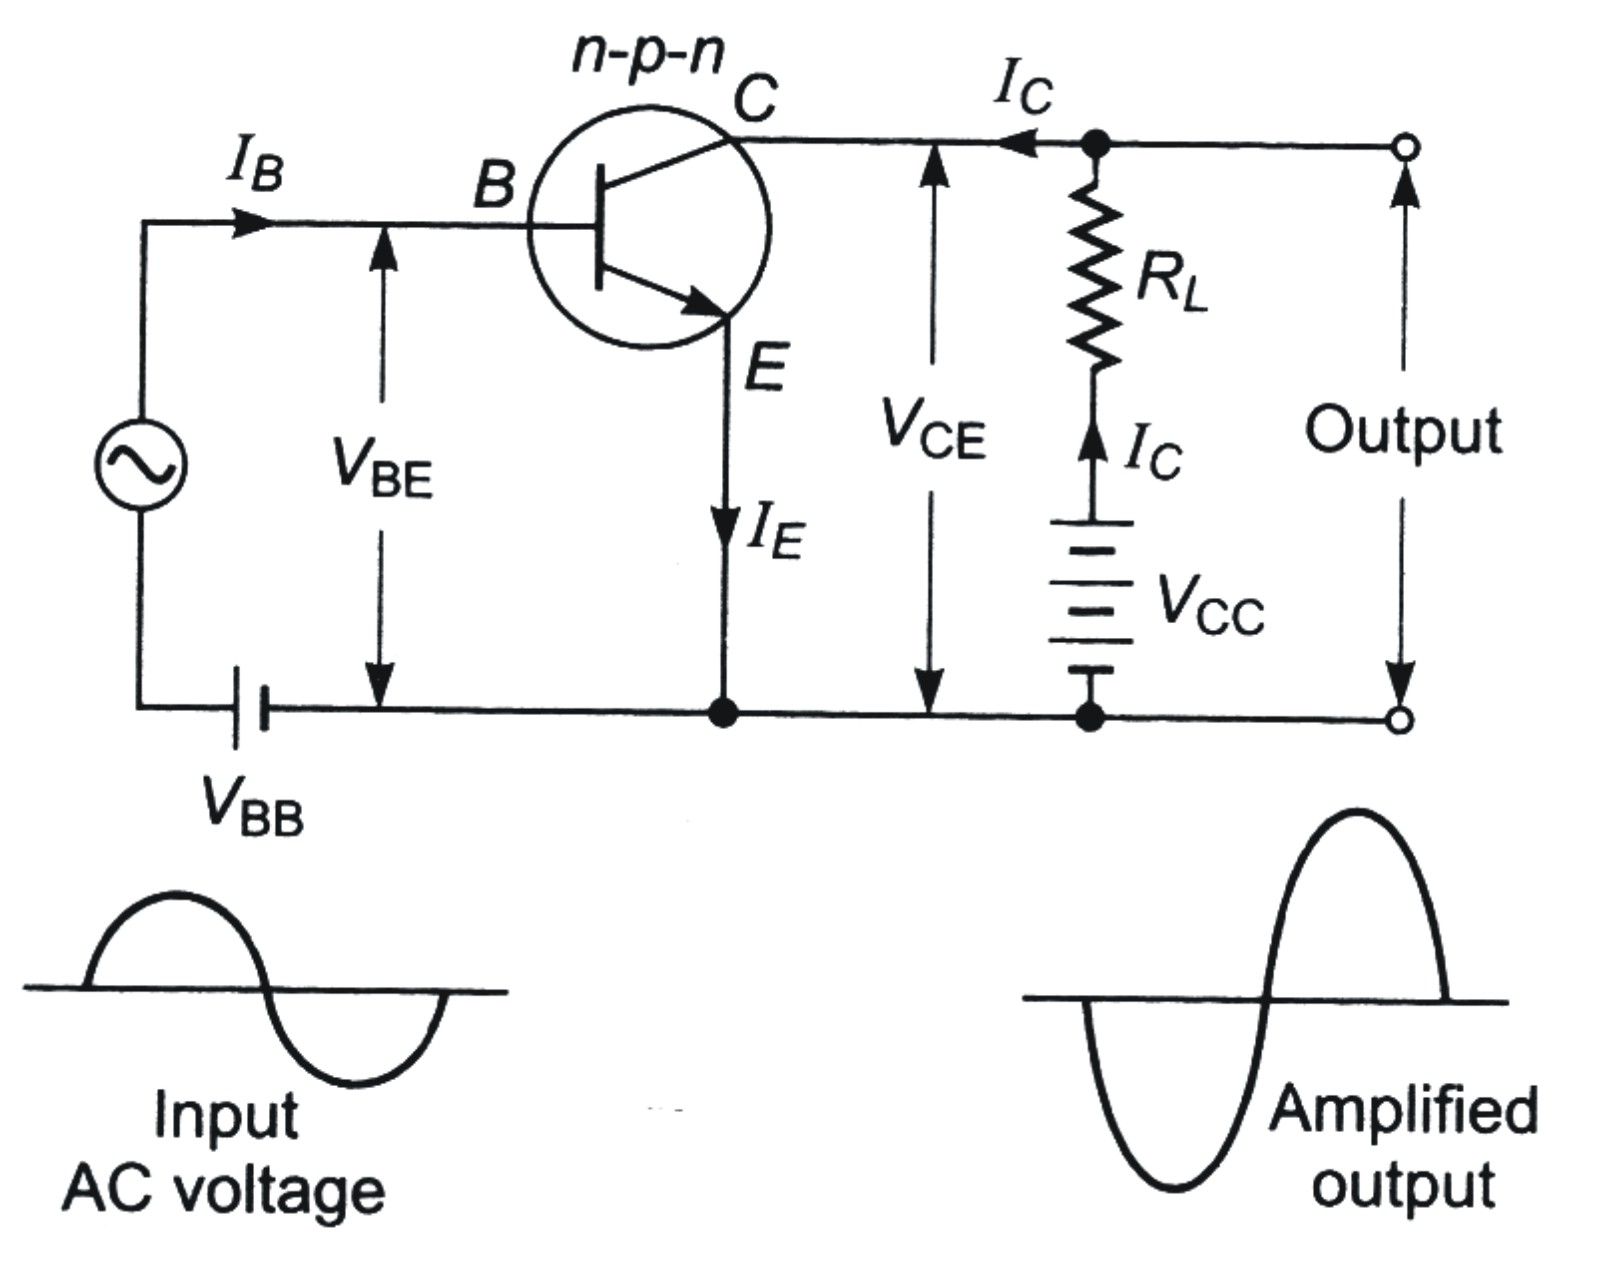
\includegraphics[width=\linewidth]{img/ce amplifier}\\
	When no signal is applied, the input ckt is FB by $ V_{BB} $ \& dc current $ I_C $ flows. This is called \textbf{zero signal collector current.}
	$$ i_C = i_c + I_C $$
	$\star$ small i($ i_c $) is for AC, large I($ I_C $) is for DC\\
	$$ V_O = -i_C R_C $$
	
	\section{DC Load line and Operating point(Q point)}
	A st. line plotted on $ I_C $ vs $ V_{CE} $ graph to calculate the value of $ I_C $ \& $ V_{CE} $ in a given circuit\\
	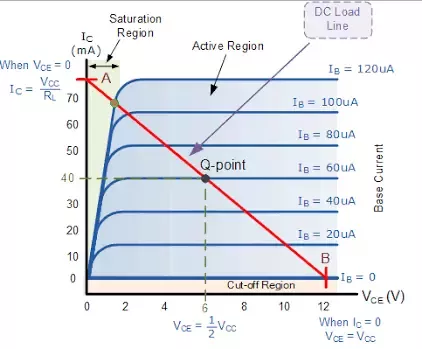
\includegraphics[width=\linewidth]{img/dc load line}\\
	Using KVL:
	$$ V_{CC} - I_CR_C - V_{CE} $$
	$$ I_C = \dfrac{-1}{R_C} V_{CE} + \dfrac{V_{CC}}{R_C} $$
	$$ y = mx + c \rightarrow\ this\ line\ is\ DC\ load\ line $$
	\begin{itemize}
		\item When $ I_B $ varies Q point also varies
		\item If BJT is used as amplifier, then Q point is selected approx in middle of load line to obtain distortion free output
	\end{itemize}
	\subsection{Instability in $ I_C $}
	$$ I_C = \beta I_B + (1+\beta) I_{CB} $$
	so, $ I_C $ is unstable due to variation in $ I_{CB} $, $ V_{BE} $, $\beta$\\
	$$ \therefore I_C = f(I_{CB}, V_{BE}, \beta) $$
	\subsubsection{due to temp}
	$ I_{C0} $ varies, $ I_C\uparrow, V_{CE} \downarrow $
	\subsubsection{Stability factor}
	$ S, S'(S_V), S''(S_\beta) $ $\rightarrow$ should be as low as possible for more stability
	$$ S = \dfrac{\partial I_C}{\partial I_{C0}} $$
	$$ S' = \dfrac{\partial I_C}{\partial V_{BE}} = S_V $$
	$$ S'' = \dfrac{\partial I_C}{\partial \beta} = S_\beta $$
	$$ \therefore \Delta I_C \approxeq \dfrac{\partial I_C}{\partial I_{C0}} \Delta I_{C0} + \dfrac{\partial I_C}{\partial V_{BE}} \Delta V_{BE} + \dfrac{\partial I_C}{\partial {\beta}} \Delta {\beta}$$
	$$ \Delta I_C \approxeq \therefore S \Delta I_{C0} + S' \Delta V_{BE} +S'' \Delta {\beta}$$
	hence, for $ I_C $ to remain stable, $ \Delta I_C $ should be small hence S, S', S'' should be small.\\
	Now, $ S = \dfrac{\partial I_C}{\partial I_{C0}} $; and $ I_C = \beta I_B + (1+\beta) I_{C0} $. Therefore:
	$$ \dfrac{\partial I_C}{\partial I_{C}} = \beta \dfrac{\partial I_B}{\partial I_{C}} + (1+\beta) \dfrac{\partial I_{C0}}{\partial I_{C}} $$
	$$ \therefore S = \dfrac{\partial I_C}{\partial I_{C0}} = \dfrac{1+\beta}{1-\beta \dfrac{\partial I_B}{\partial I_C}} $$
	Ideally, S = 1
	\subsection{Biasing techniques}
	\begin{itemize}
		\item Fixed bias ckt or Base Bias ckt
		\item C to B bias
		\item Self bias (highest stability)
	\end{itemize}

	\subsubsection{Fixed bias}
	if we need to use 1000 transistors, we would need 2000 batteries. So, we use fixed bias:\\
	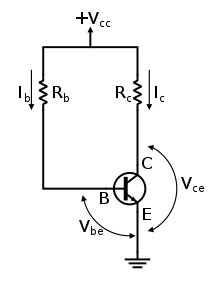
\includegraphics[width=0.5\linewidth]{img/fixed bias}\\
	$$ I_B = \dfrac{V_{CC}-V_{BE}}{R_B} $$
	since all these are fixed values, this is called fixed bias ckt
	$$ \therefore I_B = constant $$
	$$ I_C = \beta I_B, V_{CE} = V_{CC} - I_C R_C $$
	$ \dfrac{\partial I_B}{\partial I_{C}}  = 0; S = 1+\beta. So, fixed bias is unstable circuit.$
	$$ V_E = 0 $$
	$$ V_B = V_{CC} - I_B R_B $$
	$$ V_C = V_{CC} - I_C R_C $$
	$ R_C$ is selected such that $ V_C > V_B.\ So,\ V_C > V_B > V_E $ in active region
	$$ \therefore J_E\ is\ in\ FB $$
	$$ \therefore J_C\ is\ in\ RB $$

\end{document}

